\documentclass[aspectratio=169]{beamer}

\usepackage[T1]{fontenc}
\usepackage[utf8]{inputenc}
\usepackage{kotex}
\usepackage{amsmath}
\usepackage{booktabs}
\usepackage{array}
\usepackage{tikz}
\usetikzlibrary{positioning,arrows.meta}

\usetheme{Madrid}
\usecolortheme{default}
\setbeamertemplate{navigation symbols}{}
\setbeamertemplate{itemize items}[triangle]

\definecolor{Primary}{RGB}{12, 53, 106}
\definecolor{Accent}{RGB}{0, 123, 138}
\definecolor{Soft}{RGB}{244, 247, 250}

\setbeamercolor{title}{fg=Primary}
\setbeamercolor{frametitle}{fg=Primary}
\setbeamercolor{structure}{fg=Accent}
\setbeamercolor{block title}{fg=white,bg=Primary}
\setbeamercolor{block body}{bg=Soft}

\title{STM32N6 기반 낙상 감지 모델 개발}
\subtitle{Beamer 발표자료 초안}
\author{Graduate Project Team}
\institute{Falling Model Development}
\date{\today}

\begin{document}

\begin{frame}
  \titlepage
\end{frame}

\begin{frame}{프로젝트 목표}
  \begin{block}{핵심 질문}
    오프라인 성능이 아니라 \textbf{STM32N6에 실제 배포 가능한 낙상 감지 모델}을 어떻게 만들 것인가?
  \end{block}

  \begin{itemize}
    \item 입력: 자세 추정 기반 시계열 특징과 파생 기하 특징
    \item 목표: 미지 영상에서 높은 낙상 탐지율과 낮은 오경보율 확보
    \item 제약: \texttt{static shape}, \texttt{int8} 양자화, NPU 친화 연산 사용
    \item 산출물: 학습 파이프라인, 비교 기준 모델, 임베디드 배포 가능 구조
  \end{itemize}
\end{frame}

\begin{frame}{데이터셋 구성}
  \begin{columns}[T]
    \column{0.56\textwidth}
    \begin{itemize}
      \item 전체 프레임 수: \textbf{4,093,620}
      \item 전체 비디오 수: \textbf{20,380}
      \item 전체 컬럼 수: \textbf{59}
      \item 입력 특징 수: \textbf{55}
      \item 양성 프레임: \textbf{314,740}
      \item 음성 프레임: \textbf{3,778,880}
    \end{itemize}

    \column{0.44\textwidth}
    \begin{block}{특징 구성}
      \begin{itemize}
        \item 키포인트 위치/신뢰도: 51개
        \item 파생 특징: 4개
        \item 라벨: 낙상 여부
      \end{itemize}
    \end{block}
  \end{columns}
\end{frame}

\begin{frame}{문제 정의와 데이터 분할}
  \begin{block}{중요 원칙}
    프레임 단위 랜덤 분할은 누수를 일으키므로 \textbf{\texttt{video\_id} 기준 그룹 분할}이 필수입니다.
  \end{block}

  \begin{itemize}
    \item 권장 비율: Train 70\%, Validation 15\%, Test 15\%
    \item 동일 비디오의 프레임은 항상 같은 split에만 포함
    \item 추가 hold-out 세트는 최종 배포 검증 전용으로 유지
    \item 평가 기준은 랜덤 프레임 정확도가 아니라 미지 비디오 일반화 성능
  \end{itemize}
\end{frame}

\begin{frame}{입력 시퀀스 설계}
  \begin{columns}[T]
    \column{0.58\textwidth}
    \begin{itemize}
      \item 각 샘플을 \textbf{10초 클립, 15 fps}로 해석
      \item 실효 구간은 \textbf{5초에서 9초} 구간으로 고정
      \item 최종 입력 텐서 크기: \textbf{60 $\times$ 55}
      \item 장점:
      \begin{itemize}
        \item 정적 입력 형태 유지
        \item 배포 파이프라인 단순화
        \item fall onset 메타데이터 불완전 문제 완화
      \end{itemize}
    \end{itemize}

    \column{0.42\textwidth}
    \begin{center}
      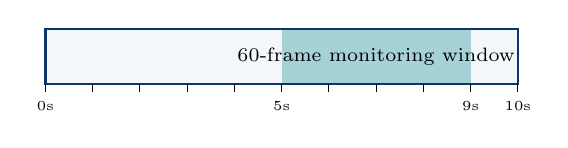
\begin{tikzpicture}[x=0.6cm,y=0.7cm]
        \fill[Soft] (0,0) rectangle (10,1);
        \fill[Accent!35] (5,0) rectangle (9,1);
        \draw[thick,Primary] (0,0) rectangle (10,1);
        \foreach \x in {0,1,...,10} {
          \draw (\x,0) -- (\x,-0.15);
        }
        \node[below] at (0,-0.15) {\tiny 0s};
        \node[below] at (5,-0.15) {\tiny 5s};
        \node[below] at (9,-0.15) {\tiny 9s};
        \node[below] at (10,-0.15) {\tiny 10s};
        \node at (7,0.5) {\scriptsize 60-frame monitoring window};
      \end{tikzpicture}
    \end{center}
  \end{columns}
\end{frame}

\begin{frame}{왜 TCN이 우선인가}
  \begin{columns}[T]
    \column{0.5\textwidth}
    \begin{block}{TCN 장점}
      \begin{itemize}
        \item \texttt{Conv1D}, \texttt{Add}, \texttt{BatchNorm}, \texttt{ReLU} 중심
        \item ONNX 변환 및 \texttt{int8} 양자화에 유리
        \item \texttt{static shape} 구조와 잘 맞음
        \item NPU 매핑 가능 연산 위주 설계 가능
      \end{itemize}
    \end{block}

    \column{0.5\textwidth}
    \begin{block}{GRU 한계}
      \begin{itemize}
        \item 연구용 성능 기준선으로는 유효
        \item 상태 처리와 런타임 제약이 큼
        \item NPU 직접 매핑이 불리함
        \item export 이후 정확도 저하 위험 존재
      \end{itemize}
    \end{block}
  \end{columns}
\end{frame}

\begin{frame}{추천 모델 아키텍처}
  \begin{block}{Primary Model: Deployment-Oriented TCN}
    \begin{itemize}
      \item 입력 형태: \texttt{(60, 55)}
      \item 깊이: 3--5 temporal convolution blocks
      \item dilation schedule: \texttt{1, 2, 4, 8}
      \item 채널 예시: \texttt{32 \textrightarrow{} 32 \textrightarrow{} 64 \textrightarrow{} 96}
      \item 활성화 함수: \texttt{ReLU}
      \item 출력 헤드: last-timestep logit 또는 pooled dense head
    \end{itemize}
  \end{block}

  \begin{block}{Secondary Model: GRU Baseline}
    \begin{itemize}
      \item 1--2 layer GRU, hidden size 32--96
      \item 목적: TCN 대비 순수 정확도 기준선 확보
    \end{itemize}
  \end{block}
\end{frame}

\begin{frame}{성능 목표와 평가 지표}
  \begin{columns}[T]
    \column{0.52\textwidth}
    \begin{block}{주요 선택 지표}
      \begin{itemize}
        \item Macro F1
        \item Fall-class Recall
        \item Fall-class Precision
        \item Video-level Detection Rate
        \item False Alarm Rate per Video
        \item Export 이후 Inference Latency
      \end{itemize}
    \end{block}

    \column{0.48\textwidth}
    \begin{block}{권장 목표치}
      \begin{itemize}
        \item Accuracy $\geq$ 95\%
        \item Recall $\geq$ 95\%
        \item Precision $\geq$ 92\%
        \item Macro F1 $\geq 0.94$
        \item Unseen-video detection $\geq$ 95\%
      \end{itemize}
    \end{block}
  \end{columns}
\end{frame}

\begin{frame}{실험 및 배포 로드맵}
  \begin{enumerate}
    \item \textbf{신뢰 가능한 baseline 구축}: grouped split, 고정 입력 구간, 재현 가능한 전처리 확립
    \item \textbf{모델 비교}: TCN과 GRU를 동일 split에서 비교
    \item \textbf{양자화 검증}: export, calibration, \texttt{int8} 정확도 저하 측정
    \item \textbf{온디바이스 정합}: 임베디드 전처리와 학습 특징 생성 일치 확인
    \item \textbf{최종 배포 평가}: 미사용 비디오와 실제 latency로 최종 선택
  \end{enumerate}
\end{frame}

\begin{frame}{예상 리스크와 대응}
  \begin{itemize}
    \item \textbf{라벨/이벤트 시점 불확실성}: 고정 모니터링 구간으로 우선 표준화
    \item \textbf{클래스 불균형}: recall과 false alarm을 함께 관리
    \item \textbf{양자화 성능 하락}: 연산자 단순화와 대표 데이터셋 기반 calibration 적용
    \item \textbf{임베디드 재현성}: 학습 특징은 반드시 디바이스에서도 계산 가능해야 함
  \end{itemize}
\end{frame}

\begin{frame}{결론}
  \begin{block}{요약}
    이 프로젝트의 핵심은 \textbf{정확도가 높은 모델}이 아니라 \textbf{STM32N6에서 실제로 돌아가는 낙상 감지 시스템}을 만드는 것입니다.
  \end{block}

  \begin{itemize}
    \item 현재 기준에서 \textbf{TCN}이 가장 현실적인 주력 아키텍처
    \item 입력은 \textbf{60 $\times$ 55} 고정 시퀀스로 표준화
    \item 평가는 \textbf{미지 비디오 기준 탐지율과 오경보율} 중심으로 수행
    \item 이후 단계는 \textbf{export, quantization, on-device 검증}까지 연결
  \end{itemize}
\end{frame}

\end{document}
